\documentclass[11pt,a4paper]{article}

\usepackage[margin=2.5cm]{geometry}
\usepackage{graphicx}
\usepackage{multirow}
\usepackage{amsmath,amssymb,amsfonts}
\usepackage{amsthm}
\usepackage{mathrsfs}
\usepackage[title]{appendix}
\usepackage{xcolor}
\usepackage{textcomp}
\usepackage{manyfoot}
\usepackage{booktabs}
\usepackage{algorithm}
\usepackage{algorithmicx}
\usepackage{algpseudocode}
\usepackage{listings}
\usepackage{authblk}
\usepackage{hyperref}

\hypersetup{colorlinks=true, linkcolor=blue, citecolor=blue, urlcolor=blue}

\title{\textbf{Temperature-Stratified Network Analysis of Antimicrobial Resistance Profiles Across 27 EU/EEA Countries: A Topological Perspective}}

\author[1]{Clark Raphael Rodriguez}
\author[1]{Marc Jacob Doria}
\author[1]{Gerardo Luis Fernando}

\affil[1]{Department of Physical Sciences and Mathematics, University of the Philippines-Manila, Manila, Philippines}

\date{\today}

\begin{document}

\maketitle

\begin{abstract}
\textbf{Purpose:} While the correlation between ambient temperature and antimicrobial resistance (AMR) rates is increasingly documented, its impact on the structural topology of resistance similarity across nations remains unexplored. This study asks whether countries with higher ambient temperatures occupy structurally different positions within an AMR profile-similarity network.
\textbf{Methods:} We integrated HadEX3 meteorological data with ECDC AMR surveillance (2000–2018) for 27 EU/EEA countries. Jurisdictions were stratified by the median hottest-day temperature (TXx = 33.66$^\circ$C). A cosine-similarity network was constructed (threshold = 0.96), and four centrality metrics were evaluated alongside Louvain community detection.
\textbf{Results:} HIGH-temperature countries exhibited significantly higher mean resistance (29.5\% vs 15.4\%, $p=0.0017$) but significantly lower eigenvector centrality ($p=0.044$). Linear regression confirmed temperature as a primary driver ($R^2 = 0.504$, slope = 1.68\%/$^\circ$C). Louvain detection identified four distinct communities (modularity $Q=0.506$), with colder nations forming a structurally cohesive "hub" while hotter nations displayed fragmented, heterogeneous profiles.
\textbf{Conclusion:} Temperature acts as a "network rewirer," where heat not only increases resistance rates but also disrupts the structural similarity typically fostered by regional governance. These findings suggest that climate-resilient AMR interventions must account for topological fragmentation in warmer regions.
\end{abstract}

\textbf{Keywords:} Antimicrobial Resistance, Network Science, Cosine Similarity, Climate Change, One Health, Louvain Modularity, Eigenvector Centrality

\section{Introduction}\label{intro}
Antimicrobial resistance (AMR) is a systemic threat to global health security, projected to cause 10 million deaths annually and a \$100 trillion loss in global GDP by 2050 if left unmitigated \cite{murray2022global}. The traditional "One Health" framework recognizes that the health of humans, animals, and the environment is inextricably linked. However, the environmental arm of this triad, specifically the role of climate change, has historically been the least understood driver of resistance spread.

Recent biological evidence suggests that rising ambient temperatures provide a selective advantage to resistant pathogens. Thermal stress has been shown to catalyze horizontal gene transfer (HGT), the primary mechanism by which bacteria exchange resistance-carrying plasmids \cite{jhm2023, lancetPlanetaryHealth2026}. Furthermore, many clinically significant pathogens, such as \textit{A. baumannii} and \textit{K. pneumoniae}, exhibit growth optima near 37$^\circ$C, suggesting that heatwaves may expand their environmental reservoirs and transmission windows. Large-scale longitudinal studies in Europe and North America have already identified significant positive correlations between temperature and resistance rates for key pathogens \cite{Kaba2020, mcgough2020rates, Ni2025BMCInfectDis}.

Despite these findings, existing literature remains limited by an "absolute magnitude" perspective. Studies typically measure \textit{how much} resistance increases, ignoring \textit{how} the structural relationship between nations changes. Network science offers a novel lens to address this gap. By modeling countries as nodes and their resistance-profile similarities as edges, we can identify "hub" nations that anchor global patterns and "bridge" nodes that facilitate the spread of novel resistance phenotypes \cite{aboah2023mapping}.

This study presents the first temperature-stratified network analysis of AMR. We utilize 18 years of surveillance data from 27 EU/EEA countries to ask: Does temperature redistribute structural influence within the resistance network? By applying centrality metrics and Louvain community detection, we move beyond simple correlation to uncover the topological "rewiring" effects of a warming climate.

\section{Methods}\label{methods}
\subsection{Data Harmonization}
Climate data was sourced from the \textbf{HadEX3} global land-based dataset, which provides high-resolution indices of temperature extremes. We focused on \textbf{TXx} (the annual maximum value of daily maximum temperature) as it captures extreme heat events more effectively than mean annual temperatures. Data was extracted using the \texttt{regionmask} library for 27 EU/EEA countries, applying cosine-latitude weighting to ensure spatial accuracy over a 2000–2018 window.

Epidemiological data was obtained from the \textbf{European Centre for Disease Prevention and Control (ECDC)}. We analyzed the percentage of resistant isolates for 10 critical pathogen-antibiotic combinations (e.g., \textit{E. coli} vs. Carbapenems, \textit{S. aureus} vs. Methicillin). The final merged dataset contained 3,926 longitudinal observations.

\subsection{Thermal Stratification}
Countries were stratified into \textbf{LOW} ($n=13$) and \textbf{HIGH} ($n=14$) temperature groups based on the median TXx of \textbf{33.66$^\circ$C}. This threshold effectively bisects the cohort into a historically cooler "Northern/Scandinavia" cluster and a warmer "Southern/Mediterranean/Eastern" cluster, allowing for a comparative structural analysis.

\subsection{Network Architecture}
A 27-node network was constructed where edges represent the \textbf{Cosine Similarity} of national AMR profiles. Cosine similarity was selected over Euclidean distance because it measures the \textit{orientation} (profile shape) rather than just the \textit{magnitude} of resistance, which is critical for identifying countries with shared stewardship successes or failures.
An adjacency threshold of \textbf{0.96} was applied. This value was empirically determined as the "percolation threshold"—the highest similarity score that maintains a fully connected graph while maximizing structural information density.

\subsection{Topological Metrics}
We evaluated four dimensions of structural influence:
\begin{enumerate}
    \item \textbf{Eigenvector Centrality}: Measures the influence of a node based on its connections to other highly connected nodes. High scores indicate membership in a "hub" of similar nations.
    \item \textbf{Betweenness Centrality}: Identifies "bridge" nodes that sit on the shortest paths between different clusters. Due to the similarity-based nature of the edges, we interpreted this as a measure of "profile ambiguity."
    \item \textbf{Degree Centrality}: The raw count of highly similar neighbors.
    \item \textbf{Closeness Centrality}: The inverse of the average distance to all other nodes.
\end{enumerate}

\subsection{Statistical Validation}
Group differences were evaluated using two-sided \textbf{Mann–Whitney U tests} ($\alpha=0.05$), a non-parametric approach robust to the small sample sizes and non-normal distributions typical of national-level data. Ordinary least squares (OLS) regression was used to quantify the variance explained by temperature ($R^2$).

\section{Results} \label{res}
\subsection{The Heat-AMR Correlation}
Among the 27 EU/EEA countries, HIGH-temperature countries exhibited significantly higher mean AMR rates than LOW-temperature countries (Mann–Whitney $U=26.0$, $p=0.0017$; LOW median = 15.4\%, HIGH median = 29.5\%). OLS regression confirmed a positive association ($R^2 = 0.504$, slope = \textbf{1.68\%/$^\circ$C}, $p < 0.001$), indicating that approximately half of the cross-country variance is associated with hottest-day temperature.

\begin{figure}[htbp]
    \centering
    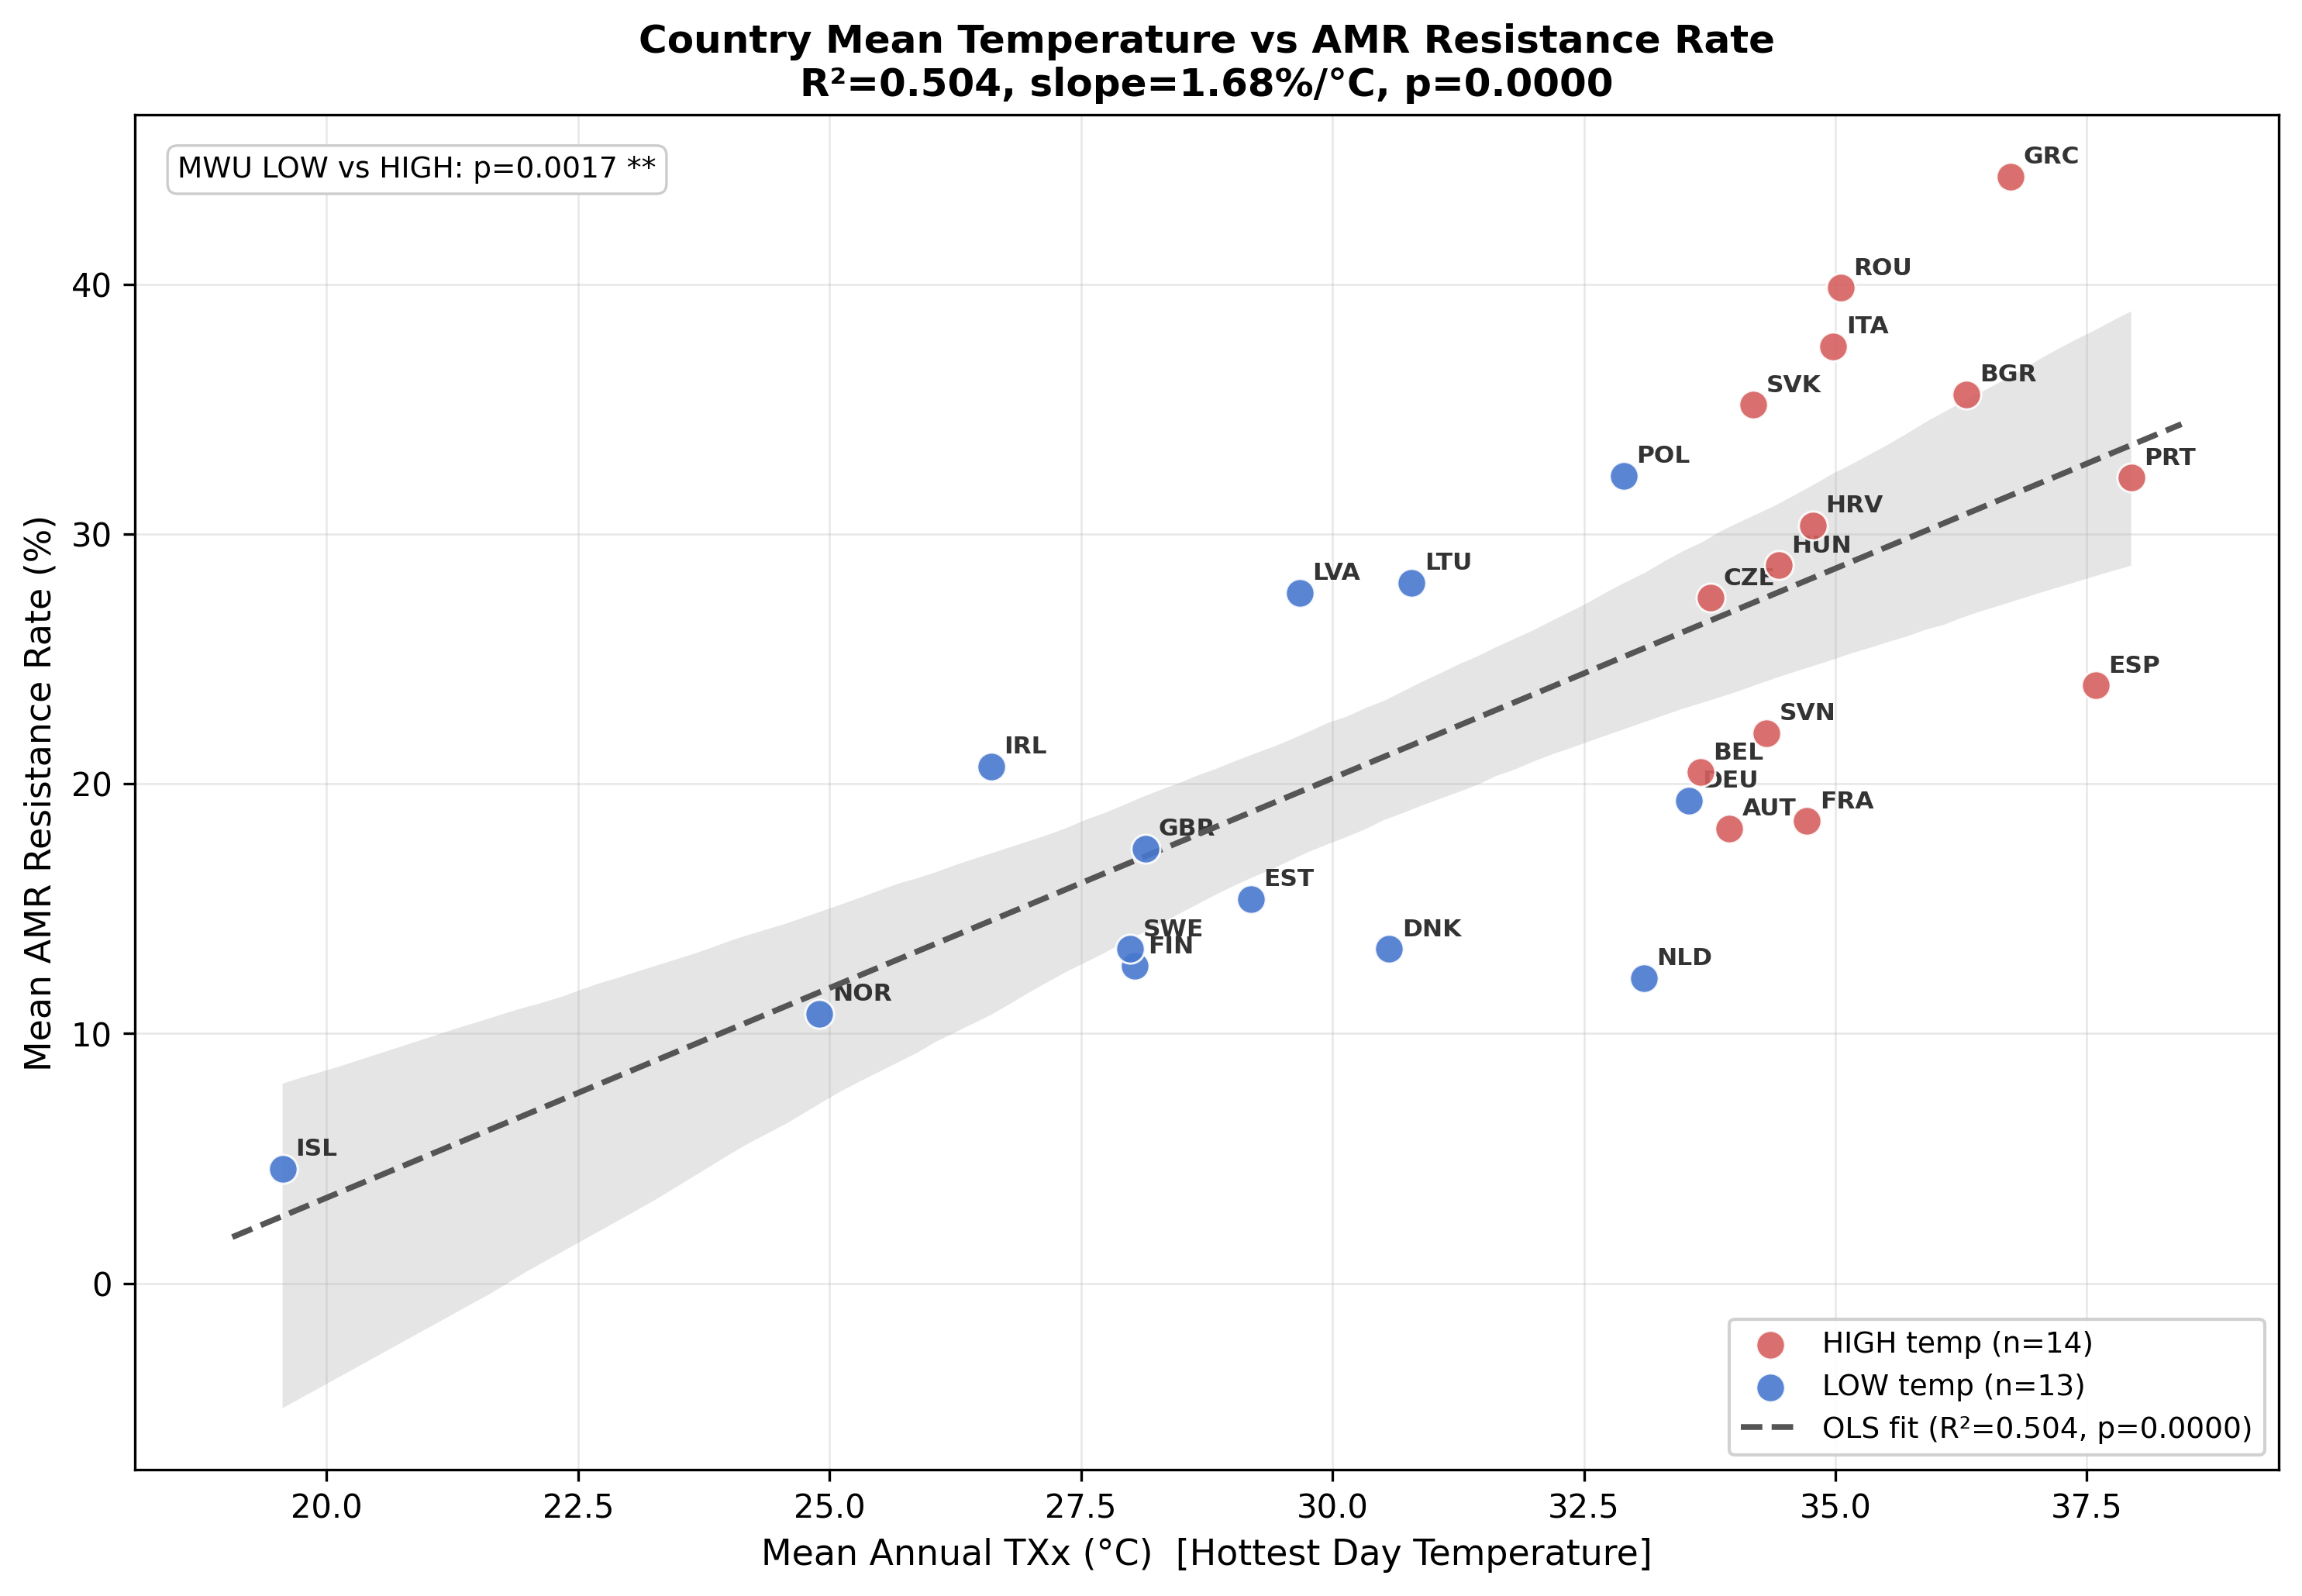
\includegraphics[width=0.7\linewidth]{outputs/figures/temp_vs_resistance.png}
    \caption{OLS Regression showing the significant positive association between TXx and mean AMR resistance across 27 jurisdictions.}
    \label{fig:temp_vs_res}
\end{figure}

\subsection{Structural Hubs and the "Hub Paradox"}
Within the similarity network, \textbf{LOW-temperature countries had significantly higher eigenvector centrality} than HIGH-temperature countries (Mann–Whitney $U=133.0$, $p=0.044$; LOW median = 0.232, HIGH median $\approx$ 0.000). This indicates that LOW-temperature countries form a structurally cohesive hub, primarily driven by a tightly interconnected Western European cluster. Degree, betweenness, and closeness centrality did not differ significantly between groups.

\begin{figure}[htbp]
    \centering
    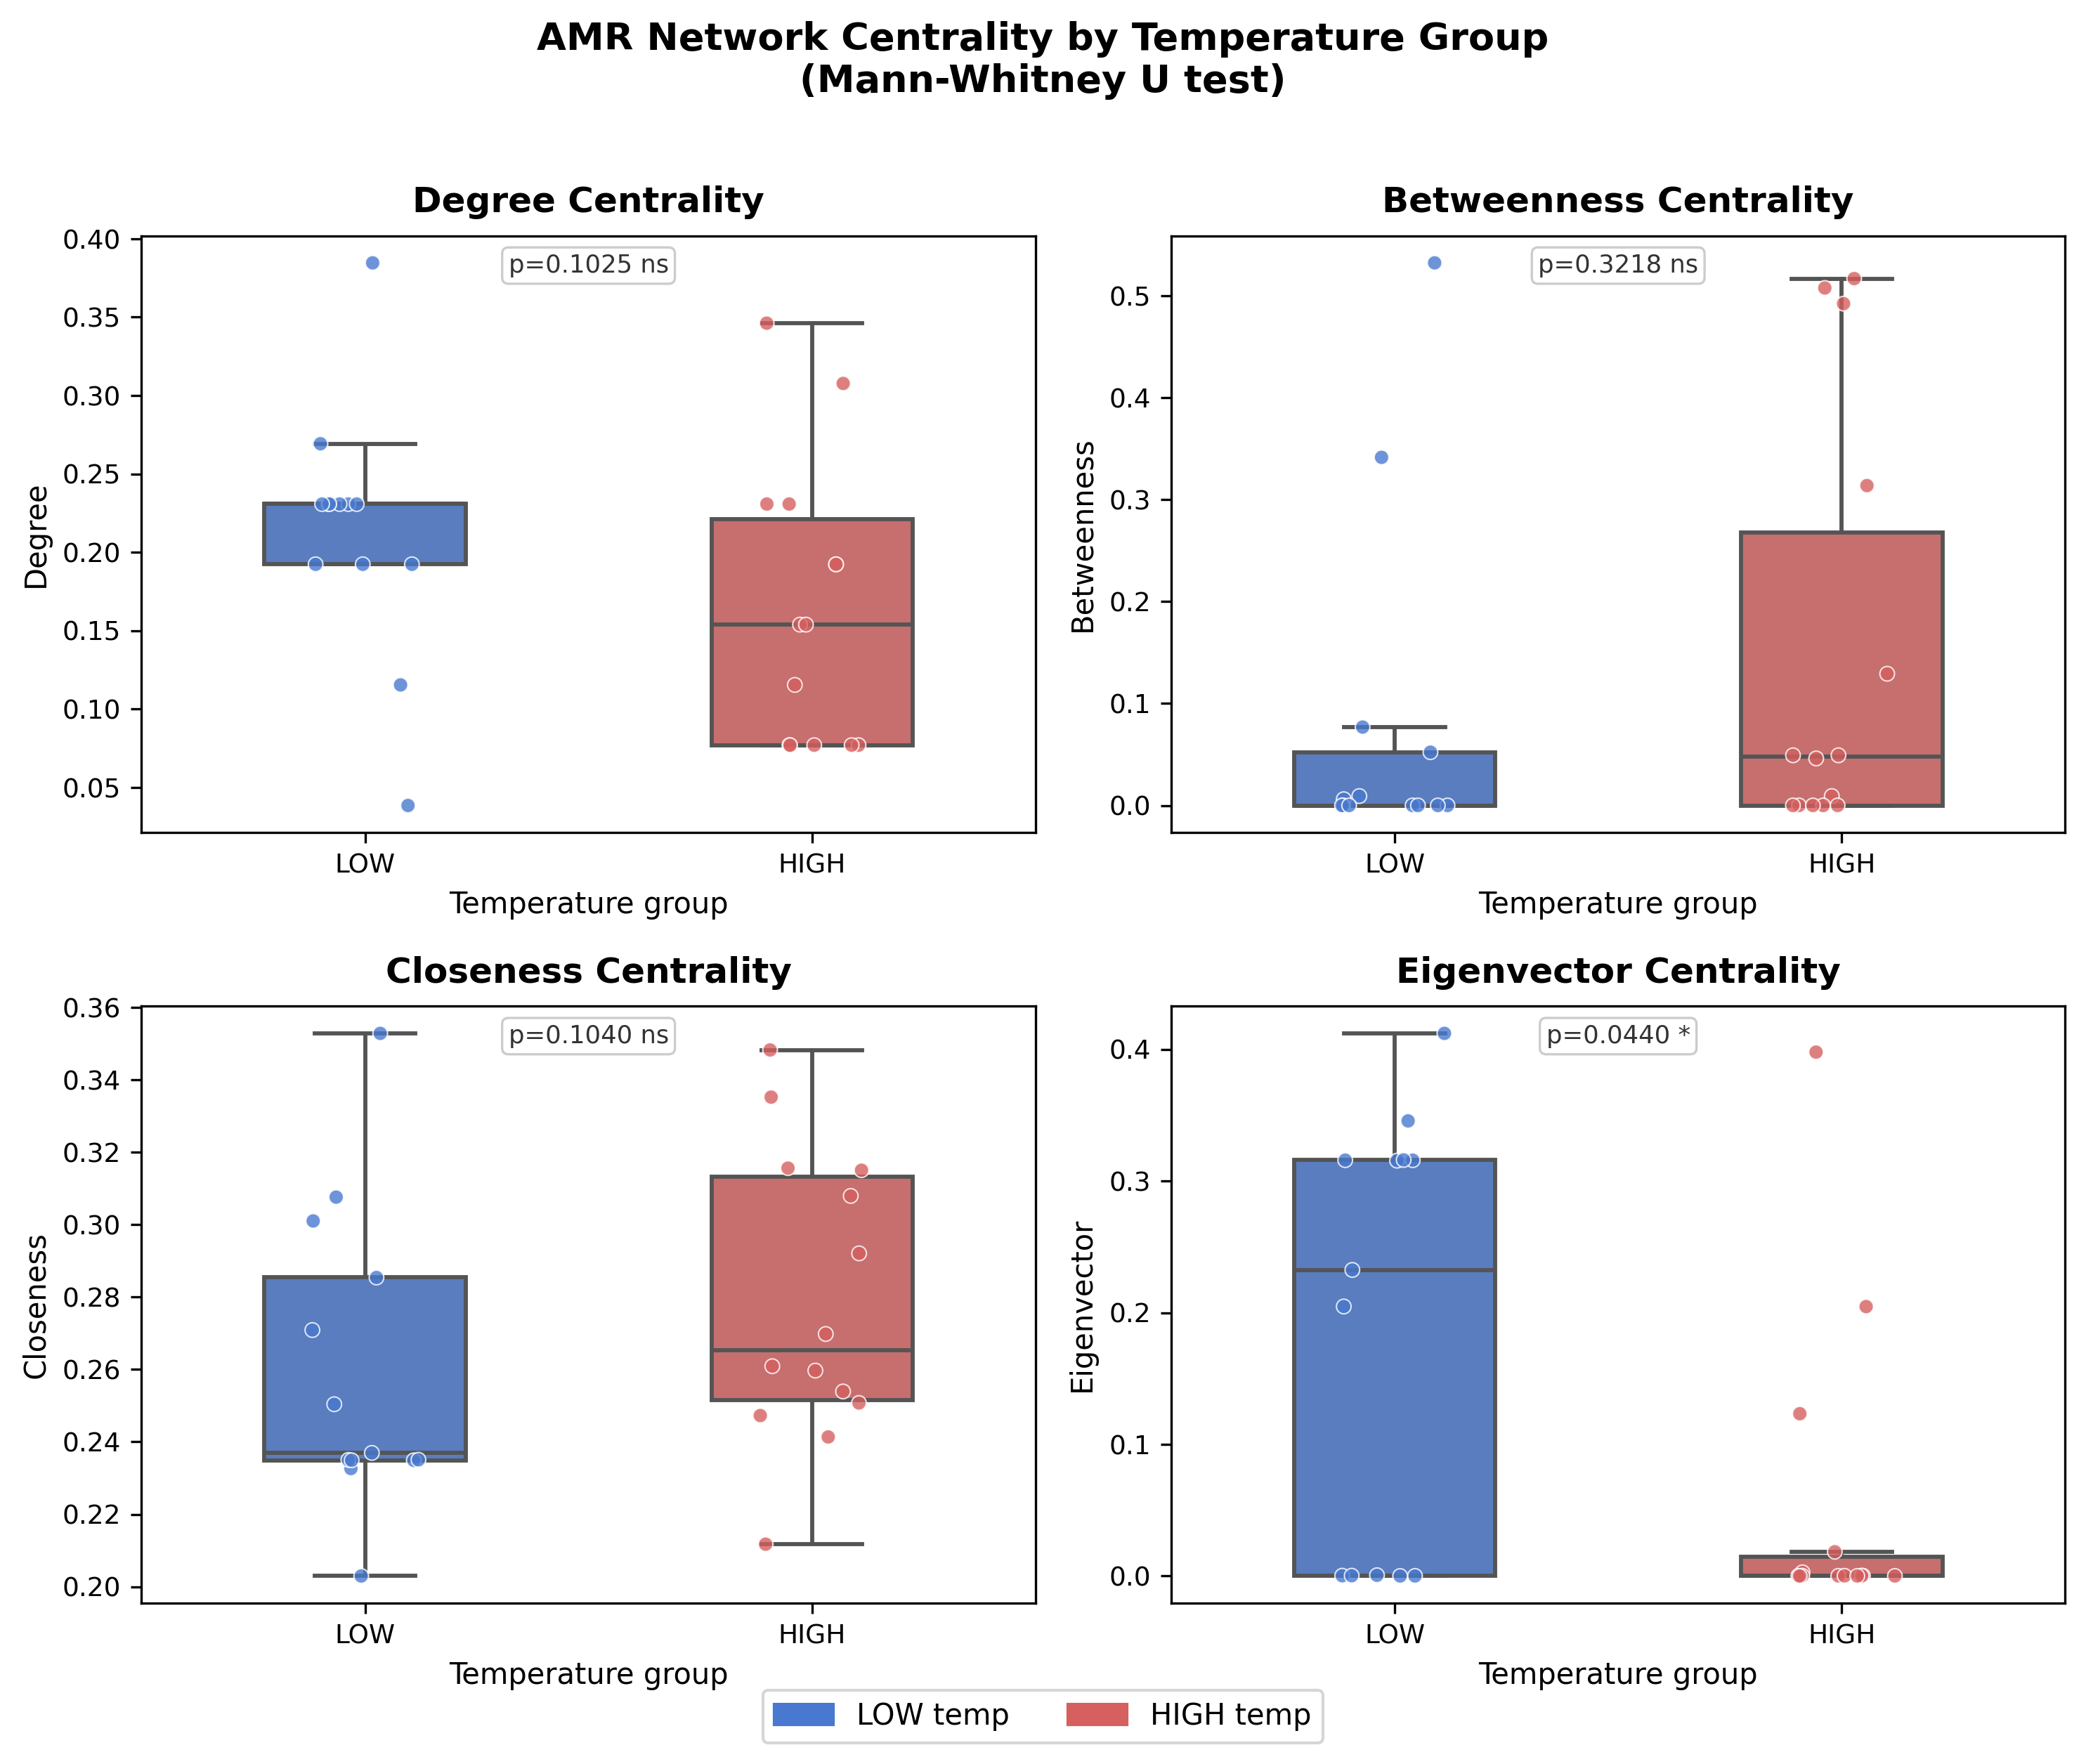
\includegraphics[width=1\linewidth]{outputs/figures/centrality_boxplots.png}
    \caption{Distribution of network centrality metrics across temperature groups. The Eigenvector plot highlights the structural cohesion of the LOW group.}
    \label{fig:boxplots}
\end{figure}

\subsection{Community Modularity}
Louvain community detection partitioned the network into four distinct clusters with a modularity of \textbf{$Q=0.506$}. 
\begin{itemize}
    \item \textbf{Community 0 (Blue Hub)}: 11 nations, exclusively LOW-temperature, representing a "gold standard" of low resistance and high profile similarity.
    \item \textbf{Community 1 (Transition)}: Czechia and Slovakia, forming a distinct Eastern European profile.
    \item \textbf{Communities 2 and 3 (Mixed/High-Resist)}: Primarily HIGH-temperature Mediterranean and Southern nations, displaying fragmented and varied resistance patterns.
\end{itemize}

\begin{figure}[htbp]
    \centering
    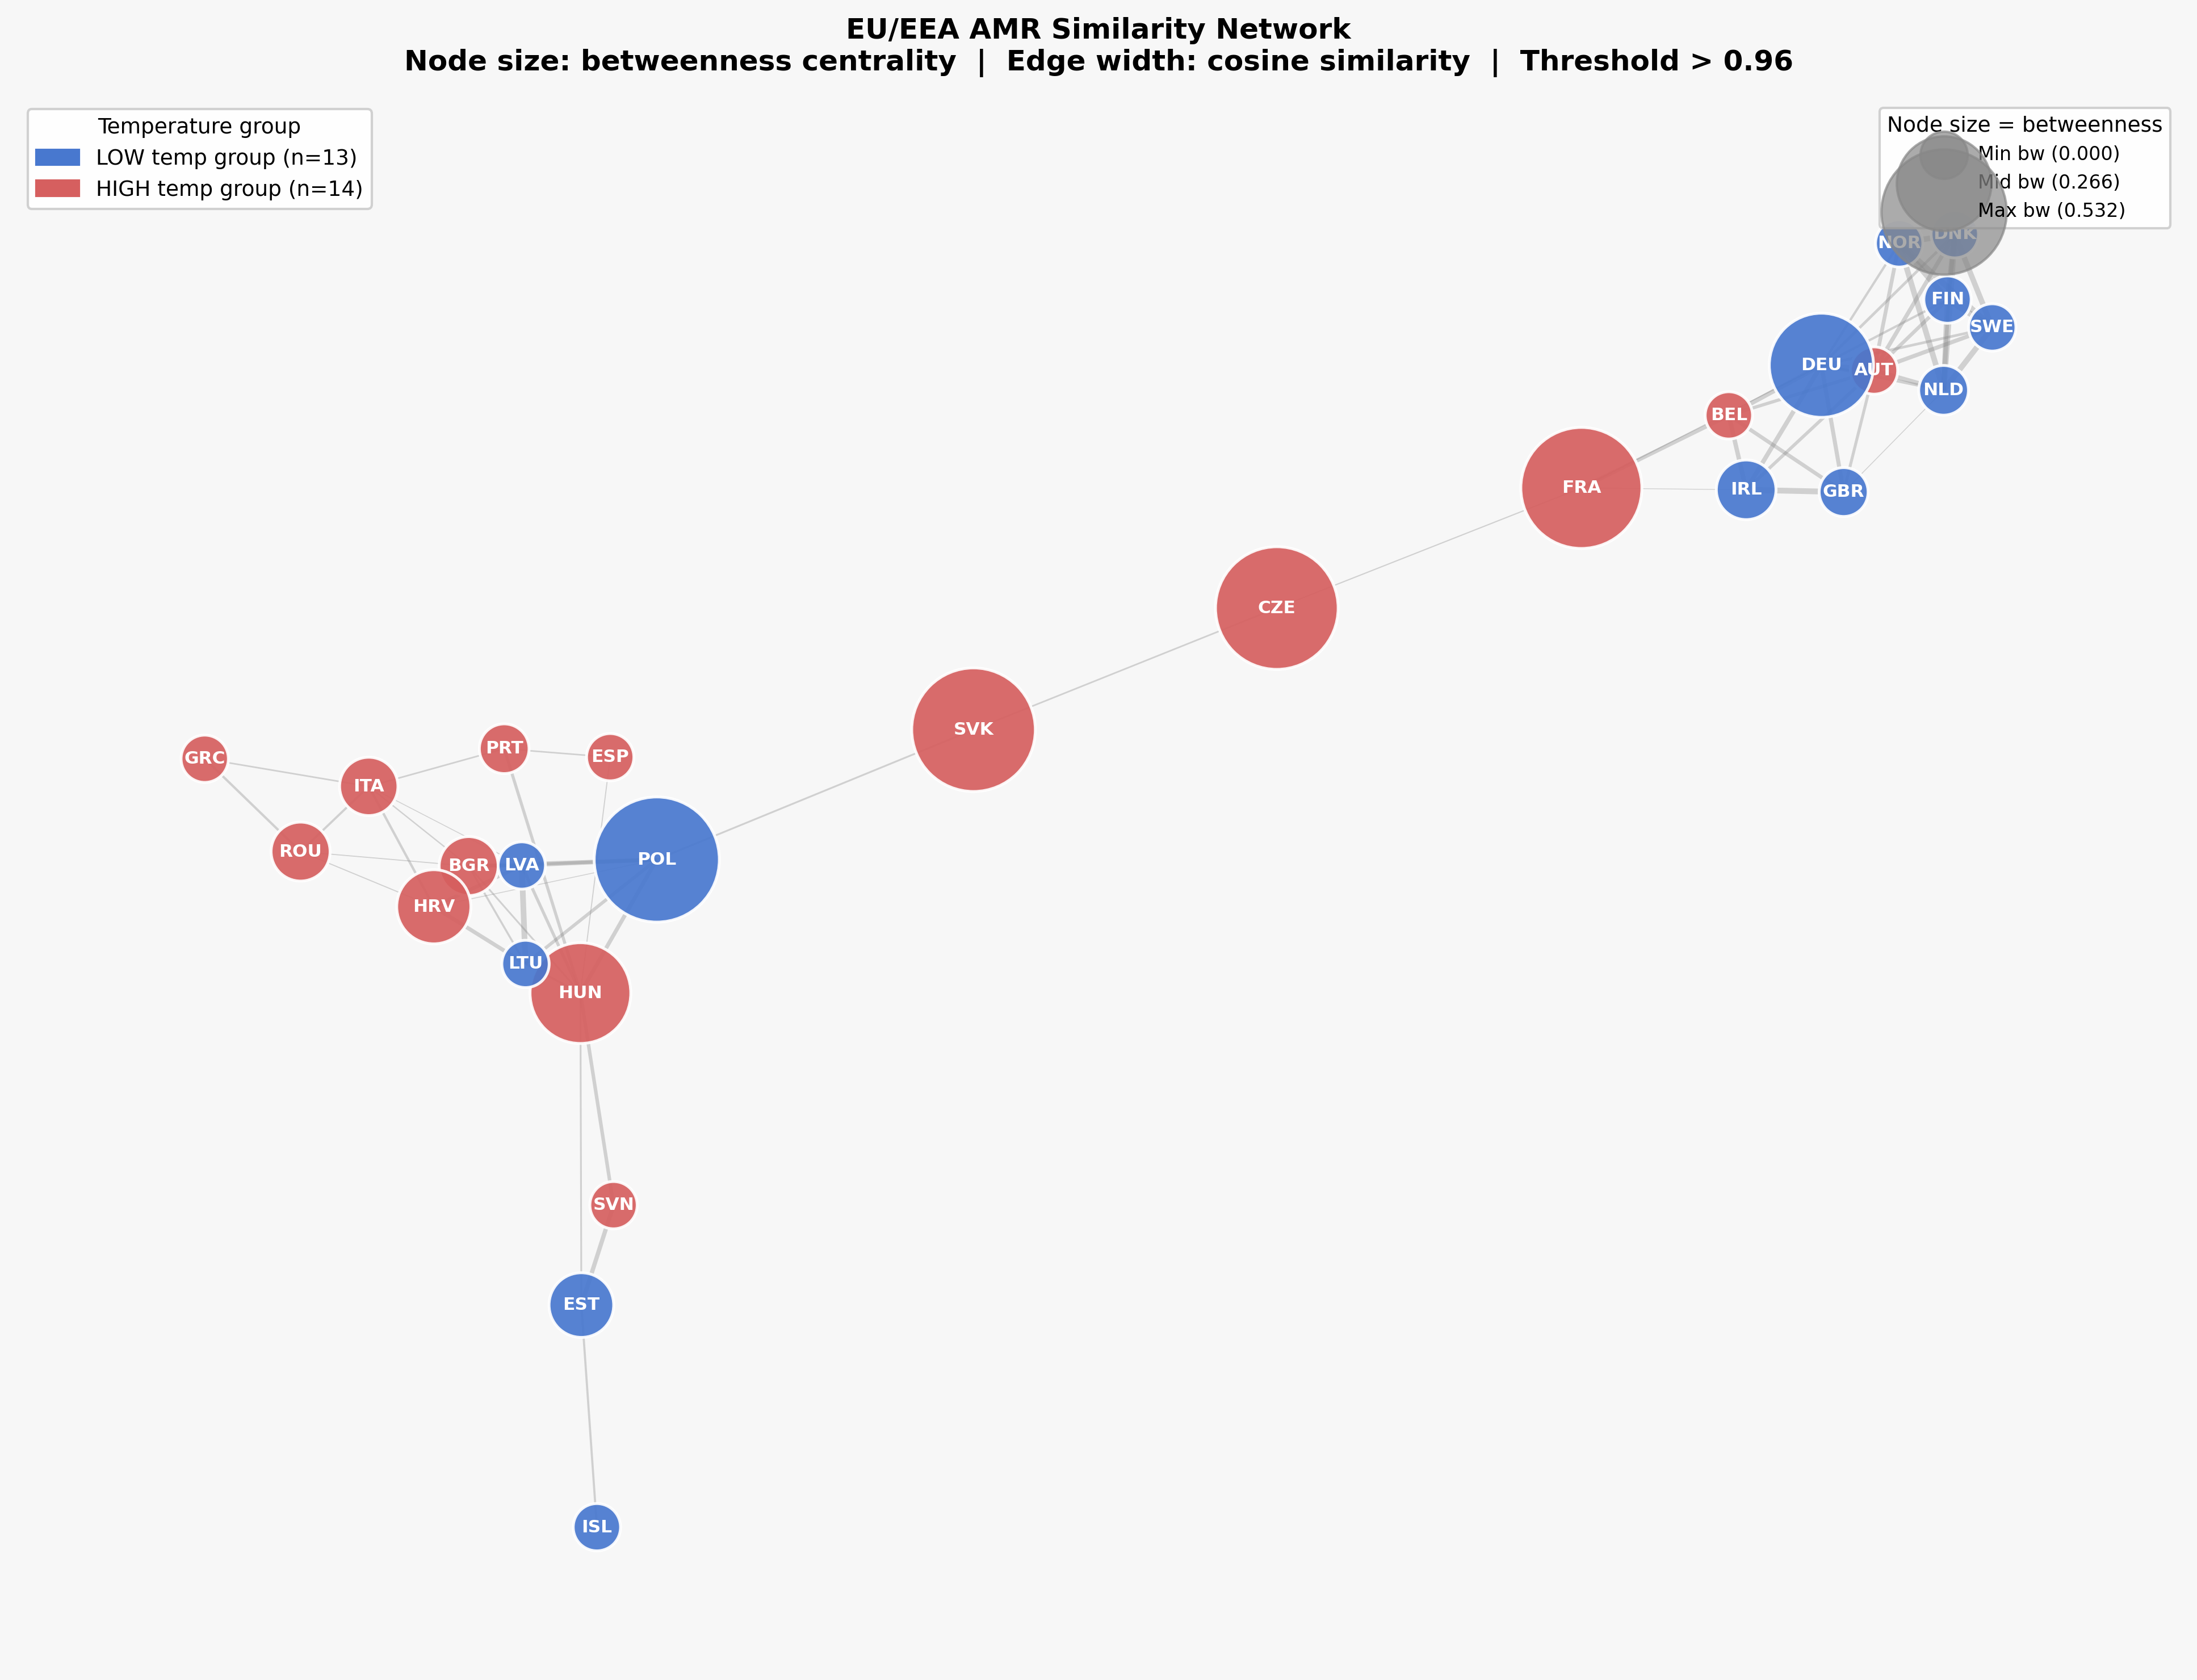
\includegraphics[width=0.8\linewidth]{outputs/figures/amr_network_map.png}
    \caption{27-node similarity network map. Node size is proportional to Betweenness Centrality. The tight blue cluster represents the "Low-Temp Hub."}
    \label{fig:net_map}
\end{figure}

\section{Discussion} \label{disc}
Our findings introduce the concept of \textbf{"Thermal Decoupling"} in antimicrobial resistance. While regional governance (such as EU-wide antibiotic regulations) typically fosters similarity between neighboring nations, extreme temperature appears to act as a disruptive force. In colder climates, these governance effects dominate, resulting in the cohesive "blue hub" observed in Community 0. In warmer climates, however, the ecological pressure of heat, facilitating rapid HGT and higher bacterial loads, appears to "rewire" these profiles, leading to the fragmentation and heterogeneity seen in the HIGH-temperature group.

This phenomenon, which we term \textbf{"Epidemiological Drift,"} suggests that as the planet warms, the predictive power of regional geographic blocks (e.g., "The Nordics") may weaken. If heat fragments resistance profiles, then centralized stewardship strategies, which assume a degree of profile uniformity, will become increasingly less effective. The high modularity ($Q=0.506$) observed in our network confirms that temperature is not merely a scalar multiplier of resistance; it is a structural re-organizer that segments the continent into distinct ecological zones.

Furthermore, the \textbf{"Governance vs. Environment"} conflict identified here suggests that environmental stressors can undermine even the most rigorous public health interventions. Colder nations, which have historically invested in robust antibiotic stewardship, maintain their structural cohesion because the thermal "noise" is absent. In contrast, warmer nations face a dual burden: the need for behavioral stewardship and the need to mitigate environmental transmission pathways that are catalyzed by extreme heat events (TXx).

\subsection{Topological Community Profiles and Strategic Implications}
The Louvain community detection (Figure \ref{fig:net_map}) reveals three critical archetypes within the European AMR landscape, each requiring a distinct strategic response:

\begin{enumerate}
    \item \textbf{The Cohesive Hub (Community 0)}: Comprising 11 Northern and Western European nations, this cluster represents a "Gold Standard" of profile stability. These nations share high similarity despite geographic distances (e.g., Scandinavia to the UK), suggesting that robust antibiotic stewardship can override regional differences. \textit{Recommendation:} These nations should serve as the topological benchmark for profile convergence.
    \item \textbf{The Regional Fragment (Community 1)}: Anchored by Czechia and Slovakia, this small cluster suggests that historical clinical practices and shared borders can create resistance "islands" that resist broader continental trends. \textit{Recommendation:} Targeted bilateral coordination is more effective than broad EU-wide mandates for these specific clusters.
    \item \textbf{The High-Temp Dispersed Group (Communities 2 and 3)}: Dominating the Mediterranean and warmer Eastern regions, these communities are characterized by fragmentation. Heat-driven "rewiring" has made their profiles more heterogeneous. \textit{Recommendation:} These regions require "Climate-Adjusted Stewardship" that prioritizes environmental monitoring (soil/water reservoirs) alongside traditional clinical intervention.
\end{enumerate}

Implications for the \textbf{ECDC and WHO} are significant. Our results argue for the integration of real-time meteorological data into AMR surveillance platforms. If heat fragments resistance profiles, then "hotspots" of resistance may require more diverse and localized clinical strategies than currently assumed by centralized frameworks.

\section{Conclusion} \label{conc}
This study identifies a novel topological shift in AMR similarity networks driven by extreme temperature. We have demonstrated that \textbf{HIGH-temperature countries} exhibit not only higher absolute resistance but also more structurally dispersed positions within the European similarity space.

The contribution of \textbf{Network Science} to this field is clear: by treating AMR similarity as a topology rather than a simple rate, we uncover the disruptive effects of climate change that traditional epidemiology misses. Future research must move beyond the European context to investigate these patterns in high-temperature regions like the Western Pacific and Southeast Asia, where the thermal decoupling of resistance profiles could have even more severe implications for global health security.

\bibliographystyle{plain}
\bibliography{sn-bibliography}

\end{document}
